\documentclass{beamer}

\usepackage{bussproofs}
\usepackage{stmaryrd}
\usepackage[utf8]{inputenc}
\usepackage{pgfpages}
\usepackage{mathtools}
\usepackage{array}
\usepackage{drs}
\input{qobitree}
\usepackage{listings}
\usepackage{cancel}
\usepackage{subcaption}
\usepackage{appendixnumberbeamer}

\setbeamertemplate{navigation symbols}{}
\setbeamertemplate{footline}
  {\hfill {\normalsize \insertframenumber{}/\inserttotalframenumber{}}}
\hypersetup{pdfstartview={Fit}}

\AtBeginSection[]
{
\begin{frame}{Outline}
  \tableofcontents[currentsection]
\end{frame}
}

\newcommand{\hsbind}{\mathbin{\gg\!=}}
\newcommand{\apl}{\mathbin{\ll\!\!\cdot}}
\newcommand{\apr}{\mathbin{\cdot\!\!\gg}}
\newcommand{\aplr}{\mathbin{\ll\!\!\cdot\!\!\gg}}
\newcommand{\cons}{\mathbin{::}}
\newcommand{\cat}{\mathbin{+\mkern-10mu+}}

\newcommand{\abs}[1]{\textsc{#1}}
\newcommand{\obj}[1]{\textbf{#1}}
\newcommand{\sem}[1]{\llbracket #1 \rrbracket}
\newcommand{\lex}[2]{\sem{\abs{#1}} &:= #2}

\newcommand{\dand}{\mathbin{\overline{\land}}}
\newcommand{\dnot}{\mathop{\overline{\lnot}}}
\newcommand{\dor}{\mathop{\overline{\lor}}}
\newcommand{\dimpl}{\mathbin{\overline{\to}}}
\newcommand{\dexists}{\mathop{\overline{\exists}}}
\newcommand{\dforall}{\mathop{\overline{\forall}}}

\newcommand{\limp}{\mathbin{{-}\mkern-3.5mu{\circ}}}

\newcommand{\llbparenthesis}{\vcenter{\hbox{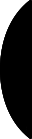
\includegraphics{symbols/llbparenthesis.png}}}}
\newcommand{\rrbparenthesis}{\vcenter{\hbox{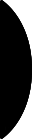
\includegraphics{symbols/rrbparenthesis.png}}}}
\newcommand{\lban}{\llparenthesis \,}
\newcommand{\rban}{\, \rrparenthesis}
\newcommand{\lbban}{\llbparenthesis \,}
\newcommand{\rbban}{\, \rrbparenthesis}
\newcommand{\banana}[1]{\lban #1 \rban}
\newcommand{\bbanana}[1]{\lbban #1 \rbban}
\newcommand{\cherry}{\rotatebox[origin=c]{270}{$\limp$}}

\newcommand{\lam}[2]{\lambda #1.\, #2}
\newcommand{\ap}[2]{#1\,#2}
\newcommand{\app}[3]{\ap{\ap{#1}{#2}}{#3}}
\newcommand{\appp}[4]{\ap{\ap{\ap{#1}{#2}}{#3}}{#4}}
\newcommand{\op}[1]{\mathtt{#1}}
\newcommand{\onto}[1]{#1 \mathalpha{:\,}}
\newcommand{\typedop}[3]{\op{#1} : #2 \rightarrowtail #3}
\newcommand{\typedopg}[3]{#1 : #2 \rightarrowtail #3}
\newcommand{\row}[2]{\{ #1 \mathrel{|} #2 \}}

\newcommand{\CC}{\mathcal{C}}
\newcommand{\FF}{\mathcal{F}}
\newcommand{\XX}{\mathcal{X}}
\newcommand{\EE}{\mathcal{E}}
\newcommand{\TT}{\mathcal{T}}
\newcommand{\PP}{\mathcal{P}}

\newcommand{\FV}{\operatorname{FV}}

\newcommand{\subst}[3]{#1[#2 \coloneqq #3]}

\newcommand{\syntclos}[1]{\mathbin{[#1]}}

\newcommand{\cibanana}{\banana{(\onto{\op{op}_i} M_i)_{i \in I},\ \onto{\eta} M_\eta}}
\newcommand{\cdbanana}{\banana{\onto{\op{op}_1} M_1,\ \dots,\ \onto{\op{op}_n} M_n,\ \onto{\eta} M_\eta}}

\newcommand{\cibbanana}{\bbanana{(\onto{\op{op}_i} M_i)_{i \in I},\ \onto{\eta} M_\eta}}

\newcommand{\TODO}[1]{\textbf{TODO}: #1}

\newcommand{\relR}{\mathbin{R}}

\newcommand{\swap}{\mathbin{\textbf{swap}}}

\newcommand{\tto}{\twoheadrightarrow}

\mathchardef\mhyphen="2D

\newcommand{\pair}[2]{\left<#1, #2\right>}
\newcommand{\inl}{\operatorname{inl}}
\newcommand{\inr}{\operatorname{inr}}

\newcommand{\true}{\textbf{T}}
\newcommand{\false}{\textbf{F}}
\newcommand{\ifte}[3]{\text{\textbf{if} $#1$ \textbf{then} $#2$ \textbf{else} $#3$}}


% Examples
\newcommand{\expr}[1]{\textsc{#1}}
\newcommand{\sume}{\expr{sum}}
\newcommand{\prode}{\expr{prod}}
\newcommand{\lite}{\expr{lit}}
\newcommand{\dive}{\expr{div}}
\newcommand{\trye}{\expr{try}}
\newcommand{\lete}{\expr{let}}
\newcommand{\vare}{\expr{var}}
\newcommand{\sumecn}[2]{\app{\sume}{#1}{#2}}
\newcommand{\prodecn}[2]{\app{\prode}{#1}{#2}}
\newcommand{\litecn}[1]{\ap{\lite}{#1}}
\newcommand{\divecn}[2]{\app{\dive}{#1}{#2}}
\newcommand{\tryecn}[2]{\app{\trye}{#1}{#2}}
\newcommand{\letecn}[3]{\appp{\lete}{\bar{#1}}{#2}{#3}}
\newcommand{\varecn}[1]{\ap{\vare}{#1}}

\newcommand{\paren}[1]{(#1)}

\newcommand{\sumec}[2]{\paren{\sumecn{#1}{#2}}}
\newcommand{\prodec}[2]{\paren{\prodecn{#1}{#2}}}
\newcommand{\litec}[1]{\paren{\litecn{#1}}}
\newcommand{\divec}[2]{\paren{\divecn{#1}{#2}}}
\newcommand{\tryec}[2]{\paren{\tryecn{#1}{#2}}}
\newcommand{\letec}[3]{\paren{\letecn{#1}{#2}{#3}}}
\newcommand{\varec}[1]{\paren{\varecn{\bar{#1}}}}


\newcommand{\NN}{\mathbb{N}}
\newcommand{\dbze}{\frac{\cdot}{0}}
\newcommand{\dbzelong}{\operatorname{DivisionByZero}}


\newcommand{\reseto}{\mathtt{reset0}}
\newcommand{\shifto}{\mathtt{shift0}}
\newcommand{\resetobanana}{\banana{\onto{\op{shift0}}{(\lam{c k}{\ap{c}{k}})}}}
\newcommand{\resetbanana}{\bbanana{\onto{\op{shift0}}{(\lam{c k}{\ap{c}{k}})}}}
\newcommand{\from}{\leftarrow}

\newcommand*{\twoheadleftrightarrow}{%
  \twoheadleftarrow
  \mathrel{\mkern-15mu}%
  \twoheadrightarrow
}

\newcommand{\ffrom}{\twoheadleftarrow}
\newcommand{\ttoffrom}{\twoheadleftrightarrow}


\newcommand{\reset}{\mathtt{reset}}
\newcommand{\shift}{\mathtt{shift}}

\newcommand{\semo}[1]{\sem{#1}_0}


\newcommand{\demph}[1]{\textbf{#1}}

\newcommand{\pipe}{\mathbin{|}}
\newcommand{\xto}[1]{\xrightarrow{#1}}

\renewcommand\theequation{\arabic{equation}}



\title{Side Effects in Natural Languages}
\author{Jirka Maršík}
\date{May 20, 2016}
\institute{Sémagramme}


\begin{document}


\begin{frame}
  \maketitle
\end{frame}


\begin{frame}{Outline}
  \tableofcontents
\end{frame}



\section{Introducing Formal Semantics}


\begin{frame}{Syllogisms}
All men are mortal. Socrates is a man. \\
$\vDash$ Socrates is mortal.
\vfill
\pause
$(\forall x.\, \obj{man}(x) \to \obj{mortal}(x)) \land
(\obj{man}(\obj{Socrates}))$ \\
$\vDash \obj{mortal}(\obj{Socrates})$
\end{frame}


\begin{frame}{The Plan}
  \begin{center}
  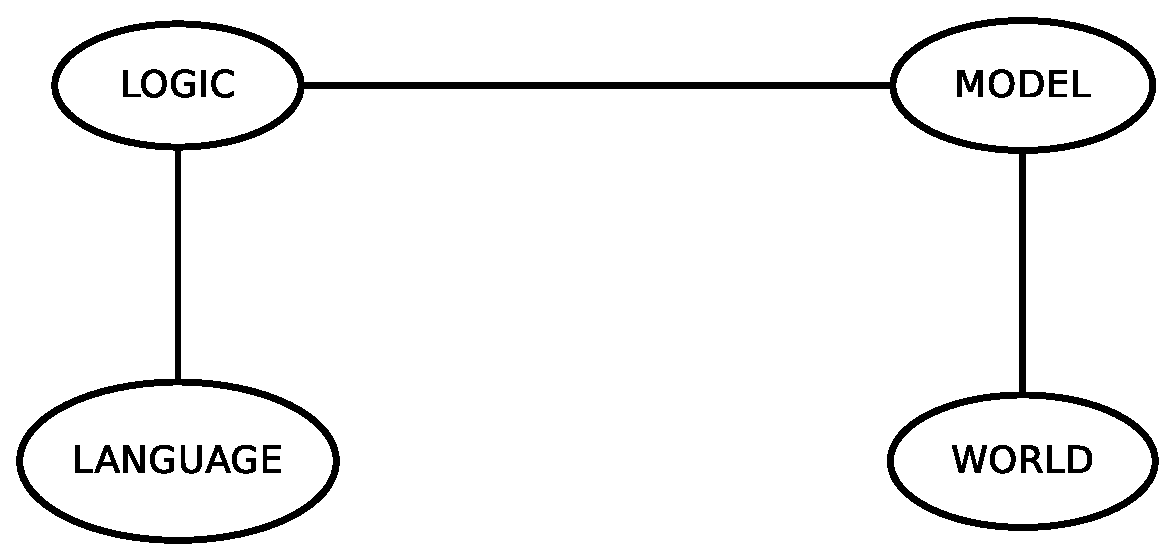
\includegraphics[width=\textheight]{plan}
  \end{center}
\end{frame}


\begin{frame}{Presuppositions}
My son is a carpenter. \\
$\vDash$ My son a carpenter. \\
$\vDash$ I have a son.
\vfill
\pause
My son is not a carpenter. \\
$\cancel{\vDash}$ My son is a carpenter. \\
$\vDash$ I have a son.
\vfill
\pause
If my son were a carpenter, he would be able to help me. \\
$\cancel{\vDash}$ My son is carpenter. \\
$\vDash$ I have a son.
\vfill
\pause
If I had a son, my son would be a carpenter. \\
$\cancel{\vDash}$ I have a son.
\end{frame}


\begin{frame}{Conventional Implicatures}
John, a swell guy, is a carpenter. \\
$\vDash$ John is a carpenter. \\
$\vDash$ John is a swell guy.
\vfill
\pause
John, a swell guy, is not a carpenter. \\
$\cancel{\vDash}$ John is a carpenter. \\
$\vDash$ John is a swell guy.
\vfill
\pause
If John, a swell guy, were a carpenter, he would be able to help me. \\
$\cancel{\vDash}$ John is a carpenter. \\
$\vDash$ John is a swell guy.
\end{frame}


\begin{frame}{Identities/Intensions}
Mary Jane loves Peter Parker but she doesn't love Spider-Man. (Peter Parker
is Spider-Man.)
\vfill
\pause
Reza doesn't believe Jesus is Jesus.
\vfill
\pause
Kim doesn't believe Sandy is Sandy. (Kim suffers from Capgras syndrome.)
\end{frame}



\section{Abstract Categorial Grammars}


\begin{frame}{Example ACG}
  $\Sigma_{\mathrm{tecto}}$
  \begin{align*}
    \abs{John}, \abs{Mary} &: NP & \abs{book}, \abs{man} &: N \\
    \abs{sleeps} &: NP \limp S & \abs{loves}, \abs{read} &: NP \limp NP \limp S \\
    \abs{some}, \abs{every} &: N \limp NP & \abs{who}, \abs{which} &: (NP \limp S) \limp N \limp N
  \end{align*}
  
  \vfill
  
  \only<2>{
  $\Sigma_{\mathrm{phono}}$
  \begin{align*}
    \syn{John}, \syn{Mary}, \syn{book}, \syn{man}, \syn{sleeps},
    \syn{loves} &: Str \\
    \syn{read}, \syn{some}, \syn{every}, \syn{who},
    \syn{which} &: Str \\
    (+) &: Str \limp Str \limp Str \\
    \epsilon &: Str
  \end{align*}
  }
  \only<3-4>{$\mathcal{L}_{\mathrm{syntax}} : \Sigma_{\mathrm{tecto}} \to \Sigma_{\mathrm{phono}}$}
  \only<3>{
  \begin{align*}
    \sem{S} &= Str \\
    \sem{NP} &= Str \\
    \sem{N} &= Str
  \end{align*}
  }
  \only<4>{
  \begin{align*}
    \sem{\abs{John}} &= \syn{John} & \sem{\abs{Mary}} &= \syn{Mary} \\
    \sem{\abs{book}} &= \syn{book} & \sem{\abs{man}} &= \syn{man} \\
    \sem{\abs{sleeps}} &= \lam{s}{s + \syn{sleeps}} & & \\
    \sem{\abs{loves}} &= \lam{o s}{s + \syn{loves} + o} & \sem{\abs{read}} &= \lam{o s}{s + \syn{read} + o} \\
    \sem{\abs{some}} &= \lam{n}{\syn{some} + n} & \sem{\abs{every}} &= \lam{n}{\syn{every} + n} \\
    \sem{\abs{who}} &= \lam{P n}{n + \syn{who} + \ap{P}{\epsilon}} & \sem{\abs{which}} &= \lam{P n}{n + \syn{which} + \ap{P}{\epsilon}}
  \end{align*}
  }
\end{frame}


\begin{frame}{Example ACG}
  \begin{align*}
  A &= \app{\abs{loves}}{\abs{Mary}}{\abs{John}} \\
  \sem{A} &= \syn{John} + \syn{loves} + \syn{Mary} \\
  \\
  B &= \app{\abs{loves}}{(\ap{\abs{some}}{(\app{\abs{who}}{(\ap{\abs{read}}{(\ap{\abs{every}}{\abs{book}})})}{\abs{man}})})}{\abs{Mary}} \\
  \sem{B} &= \syn{Mary} + \syn{loves} + \syn{some} + \syn{man} + \syn{who} + \syn{read} + \syn{every} + \syn{book} \\
  \\
  C &= \app{\abs{read}}{(\ap{\abs{every}}{(\app{\abs{which}}{(\lam{x}{\app{\abs{loves}}{x}{\abs{Mary}}})}{\abs{book}})})}{\abs{John}} \\
  \sem{C} &= \syn{John} + \syn{read} + \syn{every} + \syn{book} + \syn{which} + \syn{Mary} + \syn{loves} \\
  \end{align*}
\end{frame}



\section{Doing Formal Semantics}


\begin{frame}{Giving a Semantics to Our Fragment}
  $\Sigma_{\mathrm{tecto}}$
  \begin{align*}
    \abs{John}, \abs{Mary} &: NP & \abs{book}, \abs{man} &: N \\
    \abs{sleeps} &: NP \limp S & \abs{loves}, \abs{read} &: NP \limp NP \limp S \\
    \abs{some}, \abs{every} &: N \limp NP & \abs{who}, \abs{which} &: (NP \limp S) \limp N \limp N
  \end{align*}
  
  \vfill
  
  \only<2>{
  $\Sigma_{\mathrm{logic}}$
  \begin{align*}
    \obj{j}, \obj{m} &: \iota & \obj{man}, \obj{book} &: \iota \to o \\
    \obj{sleep} &: \iota \to o & \obj{love}, \obj{read} &: \iota \to \iota \to o \\
    (\land), (\lor), (\to) &: o \to o \to o & \lnot &: o \to o \\
    \exists, \forall &: (\iota \to o) \to o & \top, \bot &: o
  \end{align*}
  }
  \only<3-4>{
    $\mathcal{L}_{\mathrm{semantics}} : \Sigma_{\mathrm{tecto}} \to \Sigma_{\mathrm{logic}}$
  }
  \only<3>{
  \begin{align*}
    \sem{S} &= o \\
    \sem{NP} &= \iota \\
    \sem{N} &= \iota \to o
  \end{align*}
  }
  \only<4>{
  \begin{align*}
    \sem{\abs{John}} &= \obj{j} & \sem{\abs{Mary}} &= \obj{m} \\
    \sem{\abs{book}} &= \obj{book} & \sem{\abs{man}} &= \obj{man} \\
    \sem{\abs{sleeps}} &= \lam{s}{\ap{\obj{sleep}}{s}} & & \\
    \sem{\abs{loves}} &= \lam{o s}{\app{\obj{love}}{s}{o}} & \sem{\abs{read}} &= \lam{o s}{\app{\obj{read}}{s}{o}} \\
    \sem{\abs{who}}, \sem{\abs{which}} &= \lam{P n}{\lam{x}{\ap{n}{x} \land \ap{P}{x}}} \\
        \sem{\abs{some}} &=\ ??? & \sem{\abs{every}} &=\ ??? \\
  \end{align*}
  }
  \only<5-6>{
    $\mathcal{L}_{\mathrm{quantifiers}} : \Sigma_{\mathrm{tecto}} \to \Sigma_{\mathrm{logic}}$
  }
  \only<5>{
  \begin{align*}
    \sem{S} &= o \\
    \sem{NP} &= (\iota \to o) \to o \\
    \sem{N} &= \iota \to o
  \end{align*}
  }
  \only<6>{
  \begin{align*}
    \sem{\abs{John}} &= \lam{P}{\ap{P}{\obj{j}}} & \sem{\abs{Mary}} &= \lam{P}{\ap{P}{\obj{m}}} \\
    \sem{\abs{book}} &= \obj{book} & \sem{\abs{man}} &= \obj{man} \\
    \sem{\abs{sleeps}} &= \lam{S}{\ap{S}{(\lam{s}{\ap{\obj{sleep}}{s}})}} & & \\
    \sem{\abs{loves}} &= \lam{O S}{\ap{S}{(\lam{s}{\ap{O}{(\lam{o}{\app{\obj{love}}{s}{o}})}})}} \\
    \sem{\abs{read}} &= \lam{O S}{\ap{S}{(\lam{s}{\ap{O}{(\lam{o}{\app{\obj{read}}{s}{o}})}})}} \\
    \sem{\abs{who}}, \sem{\abs{which}} &= \lam{P n}{\lam{x}{\ap{n}{x} \land \ap{P}{(\lam{k}{\ap{k}{x}})}}} \\
    \sem{\abs{some}} &= \lam{n P}{\exists x.\, \ap{n}{x} \land \ap{P}{x}} \\
    \sem{\abs{every}} &= \lam{n P}{\forall x.\, \ap{n}{x} \to \ap{P}{x}}
  \end{align*}
  }
\end{frame}


\begin{frame}{Giving a Semantics to Our Fragment}
  
  \begin{align*}
  A &= \app{\abs{loves}}{\abs{Mary}}{\abs{John}} \\
  \sem{A}_{\mathrm{syn}} &= \syn{John} + \syn{loves} + \syn{Mary} \\
  \sem{A}_{\mathrm{quant}} &= \app{\obj{love}}{\obj{j}}{\obj{m}} \\
  \\
  B &= \app{\abs{loves}}{(\ap{\abs{some}}{(\app{\abs{who}}{(\ap{\abs{read}}{(\ap{\abs{every}}{\abs{book}})})}{\abs{man}})})}{\abs{Mary}} \\
  \sem{B}_{\mathrm{syn}} &= \syn{Mary} + \syn{loves} + \syn{some} + \syn{man} + \syn{who} + \syn{read} + \syn{every} + \syn{book} \\
  \sem{B}_{\mathrm{quant}} &= \exists x.\, \ap{\obj{man}}{x} \land (\forall y.\, \ap{\obj{book}}{y} \to \app{\obj{read}}{x}{y}) \land \app{\obj{love}}{\obj{m}}{x} \\
  \\
  C &= \app{\abs{read}}{(\ap{\abs{every}}{(\app{\abs{which}}{(\lam{x}{\app{\abs{loves}}{x}{\abs{Mary}}})}{\abs{book}})})}{\abs{John}} \\
  \sem{C}_{\mathrm{syn}} &= \syn{John} + \syn{read} + \syn{every} + \syn{book} + \syn{which} + \syn{Mary} + \syn{loves} \\
  \sem{C}_{\mathrm{quant}} &= \forall x.\, (\ap{\obj{book}}{x} \land \app{\obj{love}}{\obj{m}}{x}) \to \app{\obj{read}}{\obj{j}}{x}
  \end{align*}

\end{frame}


\begin{frame}{Generalizing Denotations}
  ``Upgrading'' the types of denotations in order to keep a compositional
  semantics seems like a common strategy.
  \vfill
  \begin{tabular}{llr}
    Natural Languages & Prog. Languages & Type $\alpha$ becomes \\
    \hline
    Quantification & Control &
    $(\alpha \to \omega) \to \omega$ \\
    Anaphora & State &
    $\gamma \to \alpha \times \gamma$ \\
    Intensionality & Environment &
    $\delta \to \alpha$ \\
    Presuppositions & Exceptions &
    $\alpha \oplus \chi$ \\
    Focus & &
    $\alpha \times (\alpha \to o)$ \\
    Expressives & Output &
    $\alpha \times \epsilon$ \\
    Prob. semantics & Prob. programming &
    $[\mathbb{R} \times \alpha]$ \\
  \end{tabular}
\end{frame}


\begin{frame}{Montague and Continuations}
  As we have seen, side effects and pragmatics align in their theories.
  \pause
  \vfill
  Montague's generalized quantifiers
  \begin{itemize}
  \item $\sem{NP} = (\iota \to o) \to o$
  \item e.g., the meaning of a transitive verb such as \textit{read}
    $$ \sem{\abs{read}} = \lam{S O}{\ap{S}{(\lam{s}{\ap{O}{(\lam{o}{\app{\obj{read}}{s}{o}})}})}} $$
  \end{itemize}
  \vfill
  \pause
  In computer science, discovered as continuations
  \begin{itemize}
  \item $\sem{exp_{\tau}} = (\tau \to \omega) \to \omega$
  \item e.g., applying a function $f$ to two arguments $S$ and $O$ in
    continuation-passing style
    $$\lam{P}{\ap{S}{(\lam{s}{\ap{O}{(\lam{o}{\ap{P}{(\app{f}{s}{o})}})}})}}$$
  \end{itemize}
\end{frame}


\begin{frame}{Side Effects and Pragmatics}
  \begin{columns}
    \begin{column}{0.5\textwidth}
   \begin{block}{Side Effects}
   Account for:
  \pause
  \vfill
  \begin{itemize}
  \item a program's interaction with the world of its users
    \begin{itemize}
    \item e.g., makings sounds, printing documents, moving robotic limbs\ldots
    \end{itemize}
  \end{itemize}
  \pause
  \vfill
  \begin{itemize}
  \item non-local interactions between parts of a program
    \begin{itemize}
    \item e.g., writing to and reading from variables, throwing and
      catching exceptions\ldots
    \end{itemize}
  \end{itemize}
  \end{block}
   \pause
    \end{column}
    \begin{column}{0.5\textwidth}
      \begin{block}{Pragmatics}
        Account for:
        \pause
        \vfill
        \begin{itemize}
        \item how language fits into the world of its users
          \begin{itemize}
          \item e.g., asking a colleague to print some documents\ldots
          \end{itemize}
        \pause \vfill
        \item phenomena that transcend the bounds of an isolated sentence
          \begin{itemize}
          \item e.g., the link between antecedent and pronoun, making and
            cancelling presuppositions\ldots
          \end{itemize}
        \end{itemize}
      \end{block}
    \end{column}
  \end{columns}
  \vfill
  \pause
  \alert{Side effects also align with pragmatics in their purpose.}
\end{frame}


\begin{frame}
  \frametitle{A Fistful of Types}

  $\sem{\abs{read}}$ has had many semantic types

  \vfill

  \begin{tabular}{rl}
    Naive & $\iota \to \iota \to o$ \\
    Type-raised & $((\iota \to o) \to o) \to ((\iota \to o) \to o) \to o$ \\
    Dynamic$_1$ & $((\iota \to \gamma \to (\gamma \to o) \to o) \to \gamma \to (\gamma \to o) \to o)$ \\ & $\to ((\iota \to \gamma \to (\gamma \to o) \to o) \to \gamma \to (\gamma \to o) \to o)$ \\ & $\to \gamma \to (\gamma \to o) \to o$ \\
    Dynamic$_2$ & $(((\gamma \to \iota) \to \gamma \to (\gamma \to o) \to o) \to \gamma \to (\gamma \to o) \to o)$ \\ & $\to (((\gamma \to \iota) \to \gamma \to (\gamma \to o) \to o) \to \gamma \to (\gamma \to o) \to o)$ \\ & $\to \gamma \to (\gamma \to o) \to o$ \\
    Intensional$_1$ & $\iota \to \iota \to \sigma \to o$ \\
    Intensional$_2$ & $(\sigma \to \iota) \to (\sigma \to \iota) \to \sigma \to o$ \\
    Optional & $(\iota \oplus *) \to \iota \to o$ \\
    Events & $\iota \to \iota \to \beta \to \gamma \to (\gamma \to o) \to o$
  \end{tabular}
\end{frame}


\begin{frame}
  \frametitle{For a Few Types More}
  
  \begin{align*}
    \sem{\abs{read}} &: \, ((((\sigma \to \gamma \to \iota) \to \sigma \to \gamma \to (\gamma \to o) \to o) \\
    & \to \sigma \to \gamma \to (\gamma \to o) \to o) \oplus *) \\
    & \to (((\sigma \to \gamma \to \iota) \to \sigma \to \gamma \to (\gamma \to o) \to o) \\
    & \to \sigma \to \gamma \to (\gamma \to o) \to o) \\
    & \to \beta \to \sigma \to \gamma \to (\gamma \to o) \to o \\
    \sem{\abs{read}} &: \ap{\operatorname{Dyn}}{(\ap{\operatorname{Int}}{(\ap{\operatorname{Evt}}{(\ap{\operatorname{Opt}}{(\iota \to \iota \to o)})})})} \\
    \sem{\abs{read}} & =\, ???
  \end{align*}
\end{frame}


\begin{frame}{How to Avoid Changing Denotations?}
  Different linguistic features, all in one theory \\
    $\rightarrow$ more and more elaborate types
  \vfill
  \pause
  We often have to change our minds on what is meaning
  \begin{itemize}
  \item old denotations $\rightarrow$ outdated
  \item denotations from other strands of work $\rightarrow$ incompatible
  \end{itemize}
  \pause
  \vfill
  Some solutions to this problem exist already in computer science.
\end{frame}



\section{Using a Calculus of Effects and Handlers}


\begin{frame}{Inspirations}
  Origins
  \begin{itemize}
    \item Extensible Denotational Language Specifications (Cartwright \&
      Felleisen, 1994)
    \item Handlers of Algebraic Effects (Plotkin \& Pretnar, 2009)
  \end{itemize}
  \vfill
  \pause
  Effects and Handlers Spring
  \begin{itemize}
    \item Programming with Algebraic Effects and Handlers (Bauer \&
      Pretnar, 2012)
    \item Handlers in Action (Kammar \& Lindley \& Oury, 2013)
    \item Programming and Reasoning with Algebraic Effects and Dependent
      Types (Brady, 2013)
    \item Extensible Effects -- An Alternative to Monad Transformers
      (Kiselyov \& Sabry \& Swords, 2013)
  \end{itemize}
\end{frame}

\begin{frame}{Example of the Calculus}
  $$
  E = \{\typedop{get}{1}{\NN}, \typedop{put}{\NN}{1}\}
  $$
  
  \begin{align*}
  s : \NN & \vdash \etaE{s} : \FF_E(\NN) \\
  s : \NN & \vdash \app{\op{put}}{(s + 1)}{(\lam{\_}{\etaE{s}})} : \FF_E(\NN) \\
  & \vdash \app{\op{get}}{\star}{(\lam{s}{\app{\op{put}}{(s + 1)}{(\lam{\_}{\etaE{s}})}})} : \FF_E(\NN)
  \end{align*}

  \vfill

  \begin{align*}
  \vdash \bbanana{& \onto{\op{get}}{(\lam{\_ k}{\lam{s}{\app{k}{s}{s}}})} \\
                  & \onto{\op{put}}{(\lam{s' k}{\lam{s}{\app{k}{\star}{s'}}})} \\
                  & \onto{\eta}{(\lam{x}{\lam{s}{x}})}} : \FF_E(\alpha) \to \NN \to \alpha
  \end{align*}
\end{frame}

\begin{frame}{Formal Properties}
  Subject Reduction
  \vfill
  \pause
  Confluence
  \begin{itemize}
  \item using a translation to Combinatory Reduction Systems
  \end{itemize}
  \vfill
  \pause
  Termination
  \begin{itemize}
  \item using a translation to Inductive Data Type Systems
  \end{itemize}
  \vfill
  \pause
  Strong Normalization
  \begin{itemize}
  \item corollary of the last two
  \end{itemize}
  \vfill
  \pause
  No Progress though!

  NB: All this compatible with sums and products.
\end{frame}



\appendix

\begin{frame}{Deixis}

\begin{align*}
  \abs{John}, \abs{Mary}, \abs{me} &: NP \\
  \abs{loves} &: NP \limp NP \limp S
\end{align*}

\vfill
\pause

\begin{align*}
  \lex{John}{\etaE{\obj{j}}} \\
  \lex{Mary}{\etaE{\obj{m}}} \\
  \lex{me}{\app{\op{speaker}}{\star}{(\lam{x}{\etaE{x}})}} \\
  \lex{loves}{\lam{O S}{{\obj{love}} \apr S \aplr O}}
\end{align*}

\end{frame}


\begin{frame}{Deixis in Action}

\begin{itemize}
  \item John loves Mary.
  \item Mary loves me.
\end{itemize}

\vfill
\pause

\begin{align*}
  \sem{\app{\abs{loves}}{\abs{Mary}}{\abs{John}}} & \tto 
  \etaE{(\app{\obj{love}}{\obj{j}}{\obj{m}})} \\
  \sem{\app{\abs{loves}}{\abs{me}}{\abs{Mary}}} & \tto
  \app{\op{speaker}}{\star}{(\lam{x}{\app{\obj{love}}{\obj{m}}{x}})}
\end{align*}

\vfill
\pause

\begin{align*}
  \withSpeaker &: \iota \to \FF_{\{\typedop{speaker}{1}{\iota}\} \uplus
    E}(\alpha) \to \FF_E(\alpha) \\
  \withSpeaker &= \lam{s M}{\ap{\banana{\onto{\op{speaker}}{(\lam{x k}{\ap{k}{s}})}}}{M}}
\end{align*}

\pause

$$
  \app{\withSpeaker}{s}{\sem{\app{\abs{loves}}{\abs{me}}{\abs{Mary}}}} \tto
  \etaE{(\app{\obj{love}}{\obj{m}}{s})}
$$

\end{frame}


\begin{frame}{Direct and Indirect Speech}
  
\begin{align*}
  \abs{said}_{\abs{is}} &: S \limp NP \limp S \\
  \abs{said}_{\abs{ds}} &: S \limp NP \limp S
\end{align*}

\vfill
\pause

\begin{align*}
  \sem{\abs{said}_{\abs{is}}} &= \lam{C S}{\obj{say} \apr S \aplr C} \\
                             &= \lam{C S}{S \hsbind (\lam{s}{\ap{\obj{say}}{s} \apr C})} \\
  \sem{\abs{said}_{\abs{ds}}} &= \lam{C S}{S \hsbind (\lam{s}{\ap{\obj{say}}{s} \apr (\app{\withSpeaker}{s}{C})})}
\end{align*}

\end{frame}


\begin{frame}{Direct and Indirect Speech in Action}
  
\begin{itemize}
  \item John said Mary loves me.
  \item John said, ``Mary loves me''.
\end{itemize}

\vfill
\pause

\begin{align*}
  \sem{\app{\abs{said}_{\abs{is}}}{(\app{\abs{loves}}{\abs{me}}{\abs{Mary}})}{\abs{John}}}
  & \tto \app{\op{speaker}}{\star}{(\lam{x}{\etaE{(\app{\obj{say}}{\obj{j}}{(\app{\obj{love}}{\obj{m}}{x})})}})} \\
  \sem{\app{\abs{said}_{\abs{ds}}}{(\app{\abs{loves}}{\abs{me}}{\abs{Mary}})}{\abs{John}}}
  & \tto \etaE{(\app{\obj{say}}{\obj{j}}{(\app{\obj{love}}{\obj{m}}{\obj{j}})})}
\end{align*}

\end{frame}


\begin{frame}{Quantification}
  
\begin{align*}
  \abs{every}, \abs{a} &: N \limp NP \\
  \abs{man}, \abs{woman} &: N
\end{align*}

\vfill
\pause

\begin{align*}
  \lex{every}{\lam{N}{\app{\op{scope}}{(\lam{c}{\forall \apr
          (\ap{\CC}{(\lam{x}{(N \apl x) \dimpl (\ap{c}{x})})})})}{(\lam{x}{\etaE{x}})}}} \\
  \lex{a}{\lam{N}{\app{\op{scope}}{(\lam{c}{\exists \apr
          (\ap{\CC}{(\lam{x}{(N \apl x) \dand (\ap{c}{x})})})})}{(\lam{x}{\etaE{x}})}}} \\
  \lex{man}{\etaE{\obj{man}}} \\
  \lex{woman}{\etaE{\obj{woman}}}
\end{align*}

\vfill
\pause

\begin{align*}
  \SI &= \lam{M}{\ap{\banana{\onto{\op{scope}}{(\lam{c k}{\ap{c}{k}})}}}{M}}
\end{align*}

\end{frame}


\begin{frame}{Quantification --- Changing Old Denotations }
 
\begin{align*}
  \sem{\abs{loves}} &:= \lam{O S}{\ap{\SI}{(\app{\sem{\abs{loves}}}{O}{S})}} \\
  \sem{\abs{said}_{\abs{is}}} &:= \lam{C S}{\ap{\SI}{(\app{\sem{\abs{said}_{\abs{is}}}}{C}{S})}} \\
  \sem{\abs{said}_{\abs{ds}}} &:= \lam{C S}{\ap{\SI}{(\app{\sem{\abs{said}_{\abs{ds}}}}{C}{S})}}
\end{align*}

\end{frame}


\begin{frame}{Quantification in Action}
 
\begin{itemize}
  \item Every man loves a woman.
  \item John said every woman loves me.
  \item John said, ``Every woman loves me''.
\end{itemize}

\vfill
\pause
 
\begin{align*}
  & \sem{\app{\abs{loves}}{(\ap{\abs{a}}{\abs{woman}})}{(\ap{\abs{every}}{\abs{man}})}} \nonumber \\
  & \tto \etaE{(\forall x. \ap{\obj{man}}{x} \to (\exists y. \ap{\obj{woman}}{y} \land \app{\obj{love}}{x}{y}))} \\
  & \app{\withSpeaker}{s}{\sem{\app{\abs{said}_{\abs{is}}}{(\app{\abs{loves}}{\abs{me}}{(\ap{\abs{every}}{\abs{woman}})})}{\abs{John}}}} \nonumber \\
  & \tto \etaE{(\app{\obj{say}}{\obj{j}}{(\forall x. \ap{\obj{woman}}{x} \to \app{\obj{love}}{x}{s})})} \\
  & \sem{\app{\abs{said}_{\abs{ds}}}{(\app{\abs{loves}}{\abs{me}}{(\ap{\abs{every}}{\abs{woman}})})}{\abs{John}}} \nonumber \\
  & \tto \etaE{(\app{\obj{say}}{\obj{j}}{(\forall x. \ap{\obj{woman}}{x} \to \app{\obj{love}}{x}{\obj{j}})})}
\end{align*}

\end{frame}


\begin{frame}{Conventional Implicature}
  
\begin{align*}
  \abs{appos} &: NP \limp NP \limp NP \\
  \abs{best-friend} &: NP \limp NP
\end{align*}

\vfill
\pause

\begin{align*}
  \lex{appos}{\lam{X Y}{X \hsbind (\lam{x}{\\
      & \qquad \qquad \ap{\SI}{(\etaE{x} \mathbin{\overline{=}} Y)} \hsbind (\lam{i}{\\
          & \qquad \qquad \app{\op{implicate}}{i}{(\lam{z}{\etaE{x}})}})})}} \\
  \lex{best-friend}{\lam{X}{\obj{best-friend} \apr X}}
\end{align*}

\vfill
\pause

\begin{align*}
  \accommodate &: \FF_{\{\typedop{implicate}{o}{1}\} \uplus E}(o) \to \FF_E(o) \\
  \accommodate &= \lam{M}{\ap{\banana{\onto{\op{implicate}}{(\lam{i
            k}{\etaE{i} \dand \ap{k}{\star}})}}}{M}}
\end{align*}

\end{frame}


\begin{frame}{Conventional Implicature --- Changing Old Denotations}
\begin{align*}
  \sem{\abs{said}_{\abs{ds}}} := \lam{C S}{\ap{\SI}{( & S \hsbind (\lam{s}{
        \\ & \ap{\obj{say}}{s} \apr (\app{\withSpeaker}{s}{(\ap{\accommodate}{C})})}))}}
\end{align*}
\end{frame}


\begin{frame}{Conventional Implicature in Action}
 
\begin{itemize}
  \item John, my best friend, loves every woman.
  \item Mary, everyone's best friend, loves John.
  \item A man said, ``My best friend, Mary, loves me''.
\end{itemize}

\vfill
\pause

\begin{align*}
  & \app{\withSpeaker}{s}{(\ap{\accommodate}{\\
      &\sem{\app{\abs{loves}}{(\ap{\abs{every}}{\abs{woman}})}{(\app{\abs{appos}}{\abs{John}}{(\ap{\abs{best-friend}}{\abs{me}})})}}})} \nonumber \\
  & \tto \etaE{((\obj{j} = \ap{\obj{best-friend}}{s}) \land (\forall x. \ap{\obj{woman}}{x} \to \app{\obj{love}}{\obj{j}}{x}))} \\
  & \ap{\accommodate}{\sem{\app{\abs{loves}}{\abs{John}}{(\app{\abs{appos}}{\abs{Mary}}{(\ap{\abs{best-friend}}{\abs{everyone}})})}}} \nonumber \\
  & \tto \etaE{((\forall x. \obj{m} = \ap{\obj{best-friend}}{x}) \land (\app{\obj{love}}{\obj{m}}{\obj{j}}))} \\
  & \sem{\app{\abs{said}_{\abs{ds}}}{(\app{\abs{loves}}{\abs{me}}{(\app{\abs{appos}}{(\ap{\abs{best-friend}}{\abs{me}})}{\abs{Mary}})})}{(\ap{\abs{a}}{\abs{man}})}} \nonumber \\
  & \tto \etaE{(\exists x. \ap{\obj{man}}{x} \land \app{\obj{say}}{x}{((\ap{\obj{best-friend}}{x} = \obj{m}) \land (\app{\obj{love}}{(\ap{\obj{best-friend}}{x})}{x}))})}
\end{align*}
 
\end{frame}

\end{document}
